

\tikzset{every picture/.style={line width=0.75pt}} %set default line width to 0.75pt        

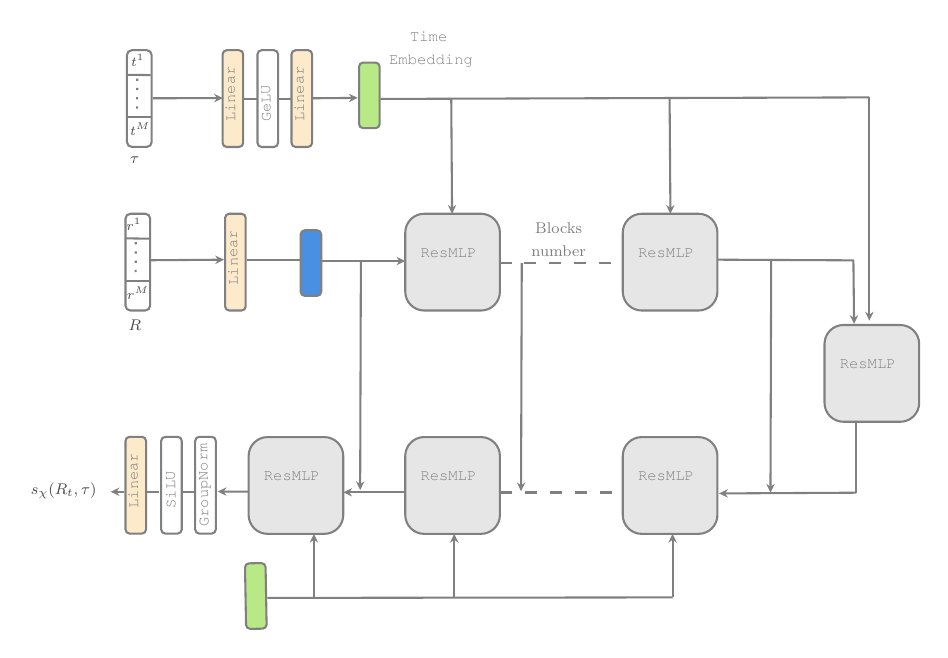
\begin{tikzpicture}[x=0.75pt,y=0.75pt,yscale=-1,xscale=1,scale=0.8]
%uncomment if require: \path (0,445); %set diagram left start at 0, and has height of 445

%Rounded Rect [id:dp45116577877352726] 
\draw  [color={rgb, 255:red, 128; green, 128; blue, 128 }  ,draw opacity=1 ][fill={rgb, 255:red, 245; green, 166; blue, 35 }  ,fill opacity=0.24 ] (121.6,35.48) .. controls (121.6,34.11) and (122.71,33) .. (124.08,33) -- (131.52,33) .. controls (132.89,33) and (134,34.11) .. (134,35.48) -- (134,88.8) .. controls (134,90.17) and (132.89,91.28) .. (131.52,91.28) -- (124.08,91.28) .. controls (122.71,91.28) and (121.6,90.17) .. (121.6,88.8) -- cycle ;

%Rounded Rect [id:dp6629173804221007] 
\draw  [color={rgb, 255:red, 128; green, 128; blue, 128 }  ,draw opacity=1 ][fill={rgb, 255:red, 255; green, 255; blue, 255 }  ,fill opacity=1 ] (142.6,35.48) .. controls (142.6,34.11) and (143.71,33) .. (145.08,33) -- (152.52,33) .. controls (153.89,33) and (155,34.11) .. (155,35.48) -- (155,88.8) .. controls (155,90.17) and (153.89,91.28) .. (152.52,91.28) -- (145.08,91.28) .. controls (143.71,91.28) and (142.6,90.17) .. (142.6,88.8) -- cycle ;

%Rounded Rect [id:dp23369966317189172] 
\draw  [color={rgb, 255:red, 128; green, 128; blue, 128 }  ,draw opacity=1 ][fill={rgb, 255:red, 245; green, 166; blue, 35 }  ,fill opacity=0.24 ] (163.1,35.48) .. controls (163.1,34.11) and (164.21,33) .. (165.58,33) -- (173.02,33) .. controls (174.39,33) and (175.5,34.11) .. (175.5,35.48) -- (175.5,88.8) .. controls (175.5,90.17) and (174.39,91.28) .. (173.02,91.28) -- (165.58,91.28) .. controls (164.21,91.28) and (163.1,90.17) .. (163.1,88.8) -- cycle ;

%Rounded Rect [id:dp47916639498650393] 
\draw  [color={rgb, 255:red, 128; green, 128; blue, 128 }  ,draw opacity=1 ][fill={rgb, 255:red, 184; green, 233; blue, 134 }  ,fill opacity=1 ] (203.77,42.93) .. controls (203.77,41.56) and (204.88,40.45) .. (206.25,40.45) -- (213.69,40.45) .. controls (215.06,40.45) and (216.17,41.56) .. (216.17,42.93) -- (216.17,77.47) .. controls (216.17,78.84) and (215.06,79.95) .. (213.69,79.95) -- (206.25,79.95) .. controls (204.88,79.95) and (203.77,78.84) .. (203.77,77.47) -- cycle ;
%Rounded Rect [id:dp16876487903558512] 
\draw  [color={rgb, 255:red, 128; green, 128; blue, 128 }  ,draw opacity=1 ][fill={rgb, 255:red, 245; green, 166; blue, 35 }  ,fill opacity=0.24 ] (123.1,133.98) .. controls (123.1,132.61) and (124.21,131.5) .. (125.58,131.5) -- (133.02,131.5) .. controls (134.39,131.5) and (135.5,132.61) .. (135.5,133.98) -- (135.5,187.3) .. controls (135.5,188.67) and (134.39,189.78) .. (133.02,189.78) -- (125.58,189.78) .. controls (124.21,189.78) and (123.1,188.67) .. (123.1,187.3) -- cycle ;

%Rounded Rect [id:dp8420620309987483] 
\draw  [color={rgb, 255:red, 128; green, 128; blue, 128 }  ,draw opacity=1 ][fill={rgb, 255:red, 74; green, 144; blue, 226 }  ,fill opacity=1 ] (168.6,143.93) .. controls (168.6,142.56) and (169.71,141.45) .. (171.08,141.45) -- (178.52,141.45) .. controls (179.89,141.45) and (181,142.56) .. (181,143.93) -- (181,178.47) .. controls (181,179.84) and (179.89,180.95) .. (178.52,180.95) -- (171.08,180.95) .. controls (169.71,180.95) and (168.6,179.84) .. (168.6,178.47) -- cycle ;
%Rounded Rect [id:dp43011173971404815] 
\draw  [color={rgb, 255:red, 128; green, 128; blue, 128 }  ,draw opacity=1 ][fill={rgb, 255:red, 245; green, 166; blue, 35 }  ,fill opacity=0.24 ] (63.1,268.31) .. controls (63.1,266.94) and (64.21,265.83) .. (65.58,265.83) -- (73.02,265.83) .. controls (74.39,265.83) and (75.5,266.94) .. (75.5,268.31) -- (75.5,321.63) .. controls (75.5,323) and (74.39,324.11) .. (73.02,324.11) -- (65.58,324.11) .. controls (64.21,324.11) and (63.1,323) .. (63.1,321.63) -- cycle ;

%Rounded Rect [id:dp7382623771259675] 
\draw  [color={rgb, 255:red, 128; green, 128; blue, 128 }  ,draw opacity=1 ][fill={rgb, 255:red, 255; green, 255; blue, 255 }  ,fill opacity=1 ] (105.1,268.31) .. controls (105.1,266.94) and (106.21,265.83) .. (107.58,265.83) -- (115.02,265.83) .. controls (116.39,265.83) and (117.5,266.94) .. (117.5,268.31) -- (117.5,321.63) .. controls (117.5,323) and (116.39,324.11) .. (115.02,324.11) -- (107.58,324.11) .. controls (106.21,324.11) and (105.1,323) .. (105.1,321.63) -- cycle ;
%Rounded Rect [id:dp740256948923222] 
\draw  [color={rgb, 255:red, 128; green, 128; blue, 128 }  ,draw opacity=1 ][fill={rgb, 255:red, 255; green, 255; blue, 255 }  ,fill opacity=1 ] (84.6,268.31) .. controls (84.6,266.94) and (85.71,265.83) .. (87.08,265.83) -- (94.52,265.83) .. controls (95.89,265.83) and (97,266.94) .. (97,268.31) -- (97,321.63) .. controls (97,323) and (95.89,324.11) .. (94.52,324.11) -- (87.08,324.11) .. controls (85.71,324.11) and (84.6,323) .. (84.6,321.63) -- cycle ;
%Rounded Rect [id:dp18399833106662933] 
\draw  [color={rgb, 255:red, 128; green, 128; blue, 128 }  ,draw opacity=1 ][fill={rgb, 255:red, 128; green, 128; blue, 128 }  ,fill opacity=0.2 ] (362.6,142.9) .. controls (362.6,136.6) and (367.7,131.5) .. (374,131.5) -- (408.2,131.5) .. controls (414.5,131.5) and (419.6,136.6) .. (419.6,142.9) -- (419.6,178.38) .. controls (419.6,184.68) and (414.5,189.78) .. (408.2,189.78) -- (374,189.78) .. controls (367.7,189.78) and (362.6,184.68) .. (362.6,178.38) -- cycle ;

%Rounded Rect [id:dp6859408399476166] 
\draw  [color={rgb, 255:red, 128; green, 128; blue, 128 }  ,draw opacity=1 ][fill={rgb, 255:red, 128; green, 128; blue, 128 }  ,fill opacity=0.2 ] (484.1,209.9) .. controls (484.1,203.6) and (489.2,198.5) .. (495.5,198.5) -- (529.7,198.5) .. controls (536,198.5) and (541.1,203.6) .. (541.1,209.9) -- (541.1,245.38) .. controls (541.1,251.68) and (536,256.78) .. (529.7,256.78) -- (495.5,256.78) .. controls (489.2,256.78) and (484.1,251.68) .. (484.1,245.38) -- cycle ;

%Rounded Rect [id:dp842740857754539] 
\draw  [color={rgb, 255:red, 128; green, 128; blue, 128 }  ,draw opacity=1 ][fill={rgb, 255:red, 128; green, 128; blue, 128 }  ,fill opacity=0.2 ] (362.6,277.4) .. controls (362.6,271.1) and (367.7,266) .. (374,266) -- (408.2,266) .. controls (414.5,266) and (419.6,271.1) .. (419.6,277.4) -- (419.6,312.88) .. controls (419.6,319.18) and (414.5,324.28) .. (408.2,324.28) -- (374,324.28) .. controls (367.7,324.28) and (362.6,319.18) .. (362.6,312.88) -- cycle ;

%Rounded Rect [id:dp10628875234333468] 
\draw  [color={rgb, 255:red, 128; green, 128; blue, 128 }  ,draw opacity=1 ][fill={rgb, 255:red, 128; green, 128; blue, 128 }  ,fill opacity=0.2 ] (231.6,277.4) .. controls (231.6,271.1) and (236.7,266) .. (243,266) -- (277.2,266) .. controls (283.5,266) and (288.6,271.1) .. (288.6,277.4) -- (288.6,312.88) .. controls (288.6,319.18) and (283.5,324.28) .. (277.2,324.28) -- (243,324.28) .. controls (236.7,324.28) and (231.6,319.18) .. (231.6,312.88) -- cycle ;

%Straight Lines [id:da15987670699550205] 
\draw [color={rgb, 255:red, 128; green, 128; blue, 128 }  ,draw opacity=1 ]   (511.1,61.42) -- (511.1,192.85) ;
\draw [shift={(511.1,195.85)}, rotate = 270] [fill={rgb, 255:red, 128; green, 128; blue, 128 }  ,fill opacity=1 ][line width=0.08]  [draw opacity=0] (5.36,-2.57) -- (0,0) -- (5.36,2.57) -- (3.56,0) -- cycle    ;
%Straight Lines [id:da39303184575868344] 
\draw [color={rgb, 255:red, 128; green, 128; blue, 128 }  ,draw opacity=1 ]   (216.6,62.35) -- (511.1,61.42) ;
%Straight Lines [id:da800059204600343] 
\draw [color={rgb, 255:red, 128; green, 128; blue, 128 }  ,draw opacity=1 ]   (390.8,61.95) -- (391.28,128.5) ;
\draw [shift={(391.3,131.5)}, rotate = 269.59] [fill={rgb, 255:red, 128; green, 128; blue, 128 }  ,fill opacity=1 ][line width=0.08]  [draw opacity=0] (5.36,-2.57) -- (0,0) -- (5.36,2.57) -- (3.56,0) -- cycle    ;
%Straight Lines [id:da7453494852796207] 
\draw [color={rgb, 255:red, 128; green, 128; blue, 128 }  ,draw opacity=1 ]   (259.3,61.95) -- (259.78,128.5) ;
\draw [shift={(259.8,131.5)}, rotate = 269.59] [fill={rgb, 255:red, 128; green, 128; blue, 128 }  ,fill opacity=1 ][line width=0.08]  [draw opacity=0] (5.36,-2.57) -- (0,0) -- (5.36,2.57) -- (3.56,0) -- cycle    ;
%Straight Lines [id:da2495969210189002] 
\draw [color={rgb, 255:red, 128; green, 128; blue, 128 }  ,draw opacity=1 ] [dash pattern={on 4.5pt off 4.5pt}]  (288.09,160.95) -- (362.09,160.95) ;
%Straight Lines [id:da8597197154488614] 
\draw [color={rgb, 255:red, 128; green, 128; blue, 128 }  ,draw opacity=1 ]   (181.12,159.96) -- (228.6,159.96) ;
\draw [shift={(231.6,159.96)}, rotate = 180] [fill={rgb, 255:red, 128; green, 128; blue, 128 }  ,fill opacity=1 ][line width=0.08]  [draw opacity=0] (5.36,-2.57) -- (0,0) -- (5.36,2.57) -- (3.56,0) -- cycle    ;
%Straight Lines [id:da33226462684386915] 
\draw [color={rgb, 255:red, 128; green, 128; blue, 128 }  ,draw opacity=1 ]   (419.6,159.16) -- (501.72,159.56) ;
%Straight Lines [id:da43782889035407124] 
\draw [color={rgb, 255:red, 128; green, 128; blue, 128 }  ,draw opacity=1 ]   (501.5,159.45) -- (501.87,194.85) ;
\draw [shift={(501.9,197.85)}, rotate = 269.4] [fill={rgb, 255:red, 128; green, 128; blue, 128 }  ,fill opacity=1 ][line width=0.08]  [draw opacity=0] (5.36,-2.57) -- (0,0) -- (5.36,2.57) -- (3.56,0) -- cycle    ;
%Straight Lines [id:da23578754948847647] 
\draw [color={rgb, 255:red, 128; green, 128; blue, 128 }  ,draw opacity=1 ]   (503.18,256.6) -- (503.18,299.49) ;
%Straight Lines [id:da8816929648715184] 
\draw [color={rgb, 255:red, 128; green, 128; blue, 128 }  ,draw opacity=1 ]   (423.6,299.92) -- (503.18,299.49) ;
\draw [shift={(420.6,299.93)}, rotate = 359.69] [fill={rgb, 255:red, 128; green, 128; blue, 128 }  ,fill opacity=1 ][line width=0.08]  [draw opacity=0] (5.36,-2.57) -- (0,0) -- (5.36,2.57) -- (3.56,0) -- cycle    ;
%Straight Lines [id:da11493937440242985] 
\draw [color={rgb, 255:red, 128; green, 128; blue, 128 }  ,draw opacity=1 ] [dash pattern={on 4.5pt off 4.5pt}]  (288.64,299.39) -- (362.64,299.39) ;
%Straight Lines [id:da869681082719342] 
\draw [color={rgb, 255:red, 128; green, 128; blue, 128 }  ,draw opacity=1 ]   (197.31,299.27) -- (231.6,299.27) ;
\draw [shift={(194.31,299.27)}, rotate = 0] [fill={rgb, 255:red, 128; green, 128; blue, 128 }  ,fill opacity=1 ][line width=0.08]  [draw opacity=0] (5.36,-2.57) -- (0,0) -- (5.36,2.57) -- (3.56,0) -- cycle    ;
%Straight Lines [id:da44612596689312034] 
\draw [color={rgb, 255:red, 128; green, 128; blue, 128 }  ,draw opacity=1 ]   (121.64,298.82) -- (136.8,298.83) ;
\draw [shift={(118.64,298.82)}, rotate = 0.04] [fill={rgb, 255:red, 128; green, 128; blue, 128 }  ,fill opacity=1 ][line width=0.08]  [draw opacity=0] (5.36,-2.57) -- (0,0) -- (5.36,2.57) -- (3.56,0) -- cycle    ;
%Straight Lines [id:da49219482761766953] 
\draw [color={rgb, 255:red, 128; green, 128; blue, 128 }  ,draw opacity=1 ]   (96.64,299.16) -- (104.87,299.16) ;
%Straight Lines [id:da744069622158885] 
\draw [color={rgb, 255:red, 128; green, 128; blue, 128 }  ,draw opacity=1 ]   (75.31,299.16) -- (83.53,299.16) ;
%Straight Lines [id:da013270848272890934] 
\draw [color={rgb, 255:red, 128; green, 128; blue, 128 }  ,draw opacity=1 ]   (57.2,298.93) -- (62.42,298.93) ;
\draw [shift={(54.2,298.93)}, rotate = 0] [fill={rgb, 255:red, 128; green, 128; blue, 128 }  ,fill opacity=1 ][line width=0.08]  [draw opacity=0] (5.36,-2.57) -- (0,0) -- (5.36,2.57) -- (3.56,0) -- cycle    ;
%Straight Lines [id:da29792639183075575] 
\draw [color={rgb, 255:red, 128; green, 128; blue, 128 }  ,draw opacity=1 ]   (136.09,159.49) -- (168.76,159.49) ;
%Straight Lines [id:da702427757163758] 
\draw [color={rgb, 255:red, 128; green, 128; blue, 128 }  ,draw opacity=1 ]   (134.64,62.13) -- (142.87,62.13) ;
%Straight Lines [id:da46605945347545785] 
\draw [color={rgb, 255:red, 128; green, 128; blue, 128 }  ,draw opacity=1 ]   (154.87,62.13) -- (163.09,62.13) ;
%Straight Lines [id:da6300259185680861] 
\draw [color={rgb, 255:red, 128; green, 128; blue, 128 }  ,draw opacity=1 ]   (175.56,61.96) -- (199.98,61.74) ;
\draw [shift={(202.98,61.71)}, rotate = 179.48] [fill={rgb, 255:red, 128; green, 128; blue, 128 }  ,fill opacity=1 ][line width=0.08]  [draw opacity=0] (5.36,-2.57) -- (0,0) -- (5.36,2.57) -- (3.56,0) -- cycle    ;
%Straight Lines [id:da8724877452780204] 
\draw [color={rgb, 255:red, 128; green, 128; blue, 128 }  ,draw opacity=1 ]   (451.99,159.2) -- (451.56,296.49) ;
\draw [shift={(451.56,299.49)}, rotate = 270.18] [fill={rgb, 255:red, 128; green, 128; blue, 128 }  ,fill opacity=1 ][line width=0.08]  [draw opacity=0] (5.36,-2.57) -- (0,0) -- (5.36,2.57) -- (3.56,0) -- cycle    ;
%Straight Lines [id:da5976028186816709] 
\draw [color={rgb, 255:red, 128; green, 128; blue, 128 }  ,draw opacity=1 ]   (301.77,161.18) -- (301.34,295.6) ;
\draw [shift={(301.33,298.6)}, rotate = 270.18] [fill={rgb, 255:red, 128; green, 128; blue, 128 }  ,fill opacity=1 ][line width=0.08]  [draw opacity=0] (5.36,-2.57) -- (0,0) -- (5.36,2.57) -- (3.56,0) -- cycle    ;
%Straight Lines [id:da1735182413440839] 
\draw [color={rgb, 255:red, 128; green, 128; blue, 128 }  ,draw opacity=1 ]   (204.88,160.49) -- (204.45,294.91) ;
\draw [shift={(204.44,297.91)}, rotate = 270.18] [fill={rgb, 255:red, 128; green, 128; blue, 128 }  ,fill opacity=1 ][line width=0.08]  [draw opacity=0] (5.36,-2.57) -- (0,0) -- (5.36,2.57) -- (3.56,0) -- cycle    ;
%Rounded Rect [id:dp5435791719991034] 
\draw  [color={rgb, 255:red, 128; green, 128; blue, 128 }  ,draw opacity=1 ][fill={rgb, 255:red, 184; green, 233; blue, 134 }  ,fill opacity=1 ] (148.1,378.86) .. controls (148.13,380.23) and (147.04,381.36) .. (145.67,381.38) -- (138.23,381.51) .. controls (136.86,381.54) and (135.73,380.45) .. (135.71,379.08) -- (135.1,344.54) .. controls (135.07,343.17) and (136.16,342.04) .. (137.53,342.02) -- (144.97,341.89) .. controls (146.34,341.86) and (147.47,342.95) .. (147.49,344.32) -- cycle ;
%Straight Lines [id:da5683776914233258] 
\draw [color={rgb, 255:red, 128; green, 128; blue, 128 }  ,draw opacity=1 ]   (148.6,362.85) -- (392.6,362.55) ;
%Straight Lines [id:da23839955840628768] 
\draw [color={rgb, 255:red, 128; green, 128; blue, 128 }  ,draw opacity=1 ]   (392.6,362.55) -- (392.6,327.28) ;
\draw [shift={(392.6,324.28)}, rotate = 90] [fill={rgb, 255:red, 128; green, 128; blue, 128 }  ,fill opacity=1 ][line width=0.08]  [draw opacity=0] (5.36,-2.57) -- (0,0) -- (5.36,2.57) -- (3.56,0) -- cycle    ;
%Straight Lines [id:da0923923318962463] 
\draw [color={rgb, 255:red, 128; green, 128; blue, 128 }  ,draw opacity=1 ]   (261.1,362.55) -- (261.1,327.28) ;
\draw [shift={(261.1,324.28)}, rotate = 90] [fill={rgb, 255:red, 128; green, 128; blue, 128 }  ,fill opacity=1 ][line width=0.08]  [draw opacity=0] (5.36,-2.57) -- (0,0) -- (5.36,2.57) -- (3.56,0) -- cycle    ;
%Straight Lines [id:da7721018720253876] 
\draw [color={rgb, 255:red, 128; green, 128; blue, 128 }  ,draw opacity=1 ]   (176.6,362.55) -- (176.6,327.28) ;
\draw [shift={(176.6,324.28)}, rotate = 90] [fill={rgb, 255:red, 128; green, 128; blue, 128 }  ,fill opacity=1 ][line width=0.08]  [draw opacity=0] (5.36,-2.57) -- (0,0) -- (5.36,2.57) -- (3.56,0) -- cycle    ;
%Rounded Rect [id:dp1551004112129395] 
\draw  [color={rgb, 255:red, 128; green, 128; blue, 128 }  ,draw opacity=1 ] (63.1,134.48) .. controls (63.1,132.83) and (64.43,131.5) .. (66.08,131.5) -- (75.02,131.5) .. controls (76.67,131.5) and (78,132.83) .. (78,134.48) -- (78,186.8) .. controls (78,188.45) and (76.67,189.78) .. (75.02,189.78) -- (66.08,189.78) .. controls (64.43,189.78) and (63.1,188.45) .. (63.1,186.8) -- cycle ;
%Straight Lines [id:da22891046032842355] 
\draw [color={rgb, 255:red, 128; green, 128; blue, 128 }  ,draw opacity=1 ]   (62.69,146.31) -- (77.33,146.51) ;
%Straight Lines [id:da8202528285215891] 
\draw [color={rgb, 255:red, 128; green, 128; blue, 128 }  ,draw opacity=1 ]   (62.97,171.74) -- (77.54,171.74) ;
%Straight Lines [id:da8432743896900226] 
\draw [color={rgb, 255:red, 128; green, 128; blue, 128 }  ,draw opacity=1 ] [dash pattern={on 0.84pt off 2.51pt}]  (69.31,148.57) -- (69.26,168.6) ;
%Rounded Rect [id:dp9973810427181078] 
\draw  [color={rgb, 255:red, 128; green, 128; blue, 128 }  ,draw opacity=1 ] (63.99,35.97) .. controls (63.99,34.32) and (65.32,32.99) .. (66.97,32.99) -- (75.91,32.99) .. controls (77.55,32.99) and (78.89,34.32) .. (78.89,35.97) -- (78.89,88.29) .. controls (78.89,89.93) and (77.55,91.27) .. (75.91,91.27) -- (66.97,91.27) .. controls (65.32,91.27) and (63.99,89.93) .. (63.99,88.29) -- cycle ;
%Straight Lines [id:da5612285806326431] 
\draw [color={rgb, 255:red, 128; green, 128; blue, 128 }  ,draw opacity=1 ]   (63.57,47.8) -- (78.22,48) ;
%Straight Lines [id:da22094837222694874] 
\draw [color={rgb, 255:red, 128; green, 128; blue, 128 }  ,draw opacity=1 ]   (63.86,73.23) -- (78.43,73.23) ;
%Straight Lines [id:da9238260217302401] 
\draw [color={rgb, 255:red, 128; green, 128; blue, 128 }  ,draw opacity=1 ] [dash pattern={on 0.84pt off 2.51pt}]  (70.2,50.06) -- (70.15,70.09) ;
%Straight Lines [id:da9054213973773921] 
\draw [color={rgb, 255:red, 128; green, 128; blue, 128 }  ,draw opacity=1 ]   (79.56,61.96) -- (118.8,61.84) ;
\draw [shift={(121.8,61.83)}, rotate = 179.83] [fill={rgb, 255:red, 128; green, 128; blue, 128 }  ,fill opacity=1 ][line width=0.08]  [draw opacity=0] (5.36,-2.57) -- (0,0) -- (5.36,2.57) -- (3.56,0) -- cycle    ;
%Straight Lines [id:da8899885040638749] 
\draw [color={rgb, 255:red, 128; green, 128; blue, 128 }  ,draw opacity=1 ]   (78.47,159.5) -- (119.47,159.19) ;
\draw [shift={(122.47,159.17)}, rotate = 179.57] [fill={rgb, 255:red, 128; green, 128; blue, 128 }  ,fill opacity=1 ][line width=0.08]  [draw opacity=0] (5.36,-2.57) -- (0,0) -- (5.36,2.57) -- (3.56,0) -- cycle    ;
%Rounded Rect [id:dp7103406473117098] 
\draw  [color={rgb, 255:red, 128; green, 128; blue, 128 }  ,draw opacity=1 ][fill={rgb, 255:red, 128; green, 128; blue, 128 }  ,fill opacity=0.2 ] (231.6,142.9) .. controls (231.6,136.6) and (236.7,131.5) .. (243,131.5) -- (277.2,131.5) .. controls (283.5,131.5) and (288.6,136.6) .. (288.6,142.9) -- (288.6,178.38) .. controls (288.6,184.68) and (283.5,189.78) .. (277.2,189.78) -- (243,189.78) .. controls (236.7,189.78) and (231.6,184.68) .. (231.6,178.38) -- cycle ;

%Rounded Rect [id:dp8954536542347509] 
\draw  [color={rgb, 255:red, 128; green, 128; blue, 128 }  ,draw opacity=1 ][fill={rgb, 255:red, 128; green, 128; blue, 128 }  ,fill opacity=0.2 ] (137.27,277.4) .. controls (137.27,271.1) and (142.37,266) .. (148.67,266) -- (182.87,266) .. controls (189.16,266) and (194.27,271.1) .. (194.27,277.4) -- (194.27,312.88) .. controls (194.27,319.18) and (189.16,324.28) .. (182.87,324.28) -- (148.67,324.28) .. controls (142.37,324.28) and (137.27,319.18) .. (137.27,312.88) -- cycle ;


% Text Node
\draw (121.86,77.64) node [anchor=north west][inner sep=0.75pt]  [font=\scriptsize,rotate=-269.05,xscale=0.7,yscale=0.7] [align=left] {{\fontfamily{pcr}\selectfont \textcolor[rgb]{0.5,0.5,0.5}{{\footnotesize Linear}}}};
% Text Node
\draw (163.36,77.64) node [anchor=north west][inner sep=0.75pt]  [font=\scriptsize,rotate=-269.05,xscale=0.7,yscale=0.7] [align=left] {{\fontfamily{pcr}\selectfont \textcolor[rgb]{0.5,0.5,0.5}{{\footnotesize Linear}}}};
% Text Node
\draw (123.36,176.14) node [anchor=north west][inner sep=0.75pt]  [font=\scriptsize,rotate=-269.05,xscale=0.7,yscale=0.7] [align=left] {{\fontfamily{pcr}\selectfont \textcolor[rgb]{0.5,0.5,0.5}{{\footnotesize Linear}}}};
% Text Node
\draw (63.36,310.47) node [anchor=north west][inner sep=0.75pt]  [font=\scriptsize,rotate=-269.05,xscale=0.7,yscale=0.7] [align=left] {{\fontfamily{pcr}\selectfont \textcolor[rgb]{0.5,0.5,0.5}{{\footnotesize Linear}}}};
% Text Node
\draw (143.86,77.64) node [anchor=north west][inner sep=0.75pt]  [font=\scriptsize,rotate=-269.05,xscale=0.7,yscale=0.7] [align=left] {{\fontfamily{pcr}\selectfont \textcolor[rgb]{0.5,0.5,0.5}{{\footnotesize GeLU}}}};
% Text Node
\draw (106.36,321.47) node [anchor=north west][inner sep=0.75pt]  [font=\tiny,rotate=-269.05,xscale=0.7,yscale=0.7] [align=left] {{\fontfamily{pcr}\selectfont \textcolor[rgb]{0.5,0.5,0.5}{{\footnotesize GroupNorm}}}};
% Text Node
\draw (370.5,151) node [anchor=north west][inner sep=0.75pt]  [xscale=0.7,yscale=0.7] [align=left] {{\footnotesize {\fontfamily{pcr}\selectfont \textcolor[rgb]{0.5,0.5,0.5}{ResMLP}}}};
% Text Node
\draw (492,218) node [anchor=north west][inner sep=0.75pt]  [xscale=0.7,yscale=0.7] [align=left] {{\footnotesize {\fontfamily{pcr}\selectfont \textcolor[rgb]{0.5,0.5,0.5}{ResMLP}}}};
% Text Node
\draw (370.5,285.5) node [anchor=north west][inner sep=0.75pt]  [xscale=0.7,yscale=0.7] [align=left] {{\footnotesize {\fontfamily{pcr}\selectfont \textcolor[rgb]{0.5,0.5,0.5}{ResMLP}}}};
% Text Node
\draw (239.5,285.5) node [anchor=north west][inner sep=0.75pt]  [xscale=0.7,yscale=0.7] [align=left] {{\footnotesize {\fontfamily{pcr}\selectfont \textcolor[rgb]{0.5,0.5,0.5}{ResMLP}}}};
% Text Node
\draw (303.6,135.5) node [anchor=north west][inner sep=0.75pt]  [xscale=0.7,yscale=0.7] [align=left] {\begin{minipage}[lt]{32.66pt}\setlength\topsep{0pt}
\begin{center}
\textcolor[rgb]{0.5,0.5,0.5}{{\footnotesize Blocks}}\\\textcolor[rgb]{0.5,0.5,0.5}{{\footnotesize  number}}
\end{center}

\end{minipage}};
% Text Node
\draw (220.6,20.06) node [anchor=north west][inner sep=0.75pt]  [xscale=0.7,yscale=0.7] [align=left] {\begin{minipage}[lt]{40.83pt}\setlength\topsep{0pt}
\begin{center}
\textcolor[rgb]{0.5,0.5,0.5}{{\footnotesize {\fontfamily{pcr}\selectfont Time}}}\\{\fontfamily{pcr}\selectfont \textcolor[rgb]{0.5,0.5,0.5}{{\footnotesize Embedding}}}
\end{center}

\end{minipage}};
% Text Node
\draw (63.64,194.18) node [anchor=north west][inner sep=0.75pt]  [font=\footnotesize,color={rgb, 255:red, 74; green, 74; blue, 74 }  ,opacity=1 ,xscale=0.7,yscale=0.7]  {$R$};
% Text Node
\draw (62.28,132.9) node [anchor=north west][inner sep=0.75pt]  [font=\scriptsize,color={rgb, 255:red, 74; green, 74; blue, 74 }  ,opacity=1 ,xscale=0.7,yscale=0.7]  {$r^{1}$};
% Text Node
\draw (62.71,174.18) node [anchor=north west][inner sep=0.75pt]  [font=\scriptsize,color={rgb, 255:red, 74; green, 74; blue, 74 }  ,opacity=1 ,xscale=0.7,yscale=0.7]  {$r^{M}$};
% Text Node
\draw (64.53,95.67) node [anchor=north west][inner sep=0.75pt]  [font=\footnotesize,color={rgb, 255:red, 74; green, 74; blue, 74 }  ,opacity=1 ,xscale=0.7,yscale=0.7]  {$\tau $};
% Text Node
\draw (65.17,34.39) node [anchor=north west][inner sep=0.75pt]  [font=\scriptsize,color={rgb, 255:red, 74; green, 74; blue, 74 }  ,opacity=1 ,xscale=0.7,yscale=0.7]  {$t^{1}$};
% Text Node
\draw (64.6,75.67) node [anchor=north west][inner sep=0.75pt]  [font=\scriptsize,color={rgb, 255:red, 74; green, 74; blue, 74 }  ,opacity=1 ,xscale=0.7,yscale=0.7]  {$t^{M}$};
% Text Node
\draw (4.83,292.23) node [anchor=north west][inner sep=0.75pt]  [font=\footnotesize,xscale=0.7,yscale=0.7]  {$\textcolor[rgb]{0.29,0.29,0.29}{s}\textcolor[rgb]{0.29,0.29,0.29}{_{\chi }}\textcolor[rgb]{0.29,0.29,0.29}{(}\textcolor[rgb]{0.29,0.29,0.29}{R_{t} ,\tau }\textcolor[rgb]{0.29,0.29,0.29}{)}$};
% Text Node
\draw (85.86,310.47) node [anchor=north west][inner sep=0.75pt]  [font=\scriptsize,rotate=-269.05,xscale=0.7,yscale=0.7] [align=left] {{\fontfamily{pcr}\selectfont \textcolor[rgb]{0.5,0.5,0.5}{{\footnotesize SiLU}}}};
% Text Node
\draw (239.5,151) node [anchor=north west][inner sep=0.75pt]  [xscale=0.7,yscale=0.7] [align=left] {{\footnotesize {\fontfamily{pcr}\selectfont \textcolor[rgb]{0.5,0.5,0.5}{ResMLP}}}};
% Text Node
\draw (145.17,285.5) node [anchor=north west][inner sep=0.75pt]  [xscale=0.7,yscale=0.7] [align=left] {{\footnotesize {\fontfamily{pcr}\selectfont \textcolor[rgb]{0.5,0.5,0.5}{ResMLP}}}};


\end{tikzpicture}
